%
% fig-kartoffel.tex
%
% (c) 2025 Prof Dr Andreas Müller
%
\begin{figure}
\centering
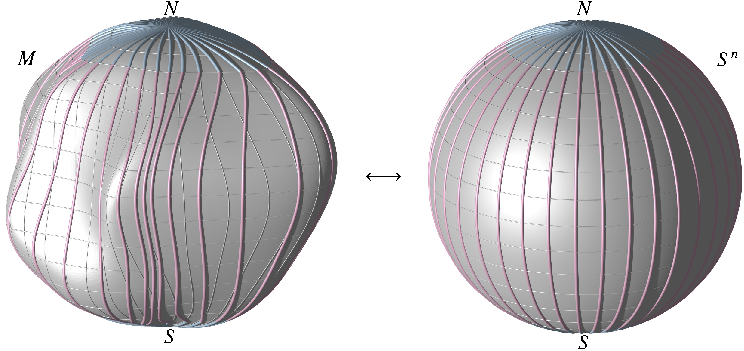
\includegraphics{chapters/120-topologie/images/sphere.pdf}
\caption{Konstruktion von Karten für eine kompakte Mannigfaltigkeit mit
einer Morse-Funktion mit genau zwei kritischen Punkten.
Ausserhalb einer Umgebung des Maximums und des Minimums können die Bahnen
(hellrot)
des Gradienten der Morse-Funktion als Koordinatenlinien (links) verwendet
und auf die Meridiane einer Kugel (rechts) abgebildet werden.
Dies zeigt, dass die Mannigfaltigkeit homömorph zu einer Kugel ist, die
Knicke zwischen den hellblauen Meridianen und den Bahnen zeigen aber auch,
dass die Mannigfaltigkeit nicht diffeomorph zu einer Kugel zu sein brauchtt.
\label{buch:topologie:morse:fig:kartoffel}}
\end{figure}
